% LTeX: language=es

\chapter{Resultados y Evaluación} \label{chap:resultados}

En este capítulo se presentan los resultados del analizador implementado. La evaluación se ha dividido en dos partes complementarias: una evaluación \textbf{cualitativa}, en la que se analiza el desempeño de la aplicación sobre vídeos reales de experimentos; y una evaluación \textbf{cuantitativa}, en la que se analiza el error cometido por el analizador con respecto al ground truth de un conjunto de vídeos generados sintéticamente.

\section{Metodología de Evaluación}

Evaluar una aplicación de visión por computador requiere disponer de una referencia con la que comparar las mediciones. En experimentos reales esto es difícil, ya que no se conoce con exactitud el diámetro o velocidad de las gotas. Para solucionar este problema, se han generado vídeos de gotas con características conocidas (ground truth), mediante una serie de scripts de evaluación desarrollados en Python.

\subsection{Scripts de evaluación}

El sistema de evaluación consta de tres scripts independientes capaces de ejecutar los experimentos de forma autónoma:

\begin{itemize}
     \item \texttt{synthetic\_video\_generator.py}: Genera los vídeos sintéticos con gotas y los ficheros CSV de ground truth. Cada gota se dibuja como un disco blanco con borde gaussiano suavizado sobre un fondo oscuro, con posición, velocidad y diámetro exactamente conocidos. Se admite la adición de ruido gaussiano y de tipo sal y pimienta de intensidad configurable. El script expone una función por experimento (\texttt{experiment\_E1\_segmentation}, \texttt{experiment\_E2\_velocity}, etc.) y puede ejecutarse directamente desde la línea de comandos indicando los experimentos deseados. Este script también se encarga de generar los ficheros CSV de ground truth, con la siguiente información: \texttt{frame}, \texttt{track\_id}, \texttt{x\_px}, \texttt{y\_px}, \texttt{diameter\_px}, \texttt{vx\_px\_frame} y \texttt{vy\_px\_frame}.
     \item \texttt{run\_experiments.py}: Ejecuta el pipeline completo de análisis. Para cada subexperimento genera los vídeos sintéticos llamando a \texttt{synthetic\_video\_generator.py}, luego se conecta directamente al backend del analizador para procesar el vídeo generado, por último compara los resultados obtenidos con el groundtruth mediante \texttt{DropletEvaluator}. Este script puede lanzar todos los experimentos o un subconjunto en particular con el argumento \texttt{--experiments}.
    \item \texttt{plot\_experiment.py}: Genera las gráficas de resultados para un único experimento a partir de su CSV de métricas. Su uso se muestra en el listing \ref{lst:plot_experiment}.
\end{itemize}

\begin{lstlisting}[language=bash, caption={Uso del script de generación de gráficas por experimento.}, label={lst:plot_experiment}]
#Generar las gráficas para el experimento E1.
python plot_experiment.py E1 --metrics_csv results/E1_metrics.csv

#Generar las gráficas para el experimento E4 con mayor resolución.
python plot_experiment.py E4 --metrics_csv results/E4_metrics.csv --dpi 300 --show
\end{lstlisting}

\subsection{Métricas de evaluación}

El evaluador calcula las siguientes métricas \cite{powers2011evaluation}\cite{everingham2010pascal} para cada vídeo analizado. El emparejamiento entre detecciones y gotas GT se realiza por distancia euclídea mínima entre centroides, con un umbral máximo de 15px:

\begin{itemize}
    \item \textbf{Precisión, Recall y F1:} Miden la tasa de detecciones correctas respecto al total de gotas presentes (GT) y al total de detecciones realizadas. Una detección se considera correcta si su centroide se encuentra a menos de 15~px del centroide GT más cercano.
    \item \textbf{MRE\textsubscript{diam}:} Error Relativo Medio del diámetro, definido como $\text{MRE} = \frac{1}{N}\sum_{i=1}^{N}\frac{|d_i^{\text{det}} - d_i^{\text{GT}}|}{d_i^{\text{GT}}}$.
    \item \textbf{RMSE\textsubscript{diam}:} Raíz del Error Cuadrático Medio del diámetro en píxeles.
    \item \textbf{Circularidad media:} Media y desviación estándar de la circularidad detectada, que en gotas sintéticas perfectamente circulares debería ser próxima a 1.
    \item \textbf{MRE\textsubscript{vel} y RMSE\textsubscript{vel}:} Error relativo y RMSE de la magnitud de velocidad detectada respecto a la velocidad GT.
    \item \textbf{Tasa de fragmentación:} Definida como $\frac{N_{\text{tracks det}} - N_{\text{tracks GT}}}{N_{\text{tracks GT}}}$, indica si el tracker divide una única trayectoria real en varios tracks.
\end{itemize}

\subsection{Evaluación cuantitativa}

\subsection{E1 - Precisión de segmentación con diámetros conocidos}
 
\textbf{Configuración:} Se generaron vídeos de 30 frames con 4 gotas estáticas por frame en cuadrícula, sin ruido, para 7 diámetros distintos: 6, 10, 15, 20, 30, 40 y 50~px. Al ser gotas estáticas e idealmente circulares, este experimento aísla el error puro de la etapa de segmentación y medición, sin la influencia del tracking ni del ruido.

En la figura \ref{fig:E1} se muestra un frame del vídeo generado para este experimento.
\begin{figure}[H]
    \centering
    
\includegraphics[width=0.4\textwidth]{figures/E1.png}
    \caption{Frame de uno de los vídeos generado para E1.}
    \label{fig:E1}
\end{figure}


\begin{table}[H]
\centering
\small
\caption{Resultados del experimento E1 (precisión de segmentación).}
\begin{tabular}{ccccccc}
\hline
\textbf{Diámetro GT (px)} & \textbf{Recall} & \textbf{Precision} & \textbf{F1} & \textbf{MRE\textsubscript{diam} (\%)} & \textbf{RMSE\textsubscript{diam} (px)} & \textbf{Circ. media} \\
\hline
6  & 1.00 & 1.00 & 1.00 & 62.32 & 3.74 & 0.8612 \\
10 & 1.00 & 1.00 & 1.00 & 39.12 & 3.91 & 0.8786 \\
15 & 1.00 & 1.00 & 1.00 & 23.72 & 3.56 & 0.9003 \\
20 & 1.00 & 1.00 & 1.00 & 19.19 & 3.84 & 0.8774 \\
30 & 1.00 & 1.00 & 1.00 & 12.93 & 3.88 & 0.8579 \\
40 & 1.00 & 1.00 & 1.00 & 9.64  & 3.86 & 0.8962 \\
50 & 1.00 & 1.00 & 1.00 & 7.73  & 3.87 & 0.8793 \\
\hline
\end{tabular}
\label{tab:e1_resultados}
\end{table}

Como se pueden observar en los resultados mostrados en la tabla \ref{tab:e1_resultados} y en la figura \ref{fig:E1_metrics}, el analizador detecta correctamente todas las gotas (Recall y Precision de 1.00) para todos los diámetros, lo que indica que la segmentación es robusta incluso para gotas pequeñas. Sin embargo, se observa un error absoluto constante en la segmentación de aproximadamente 3.8 píxeles, debido a la discretización digital y umbralización, que también explica por qué la métrica de circularidad se penaliza por el efecto escalera de los bordes perimetrales mientras que la redondez se mantiene excelente por encima de 0.95. Aunque este ensanchamiento sistemático del contorno es prácticamente despreciable en gotas grandes (reduciendo el error relativo al 7.7\% en diámetros de 50 px), resulta un factor crítico al evaluar las microgotas de 6 px, cuyo tamaño se sobreestima en más de un 62\%.

\begin{figure}[htbp]
    \centering
        
    \begin{subfigure}[b]{0.7\textwidth}
        \centering
        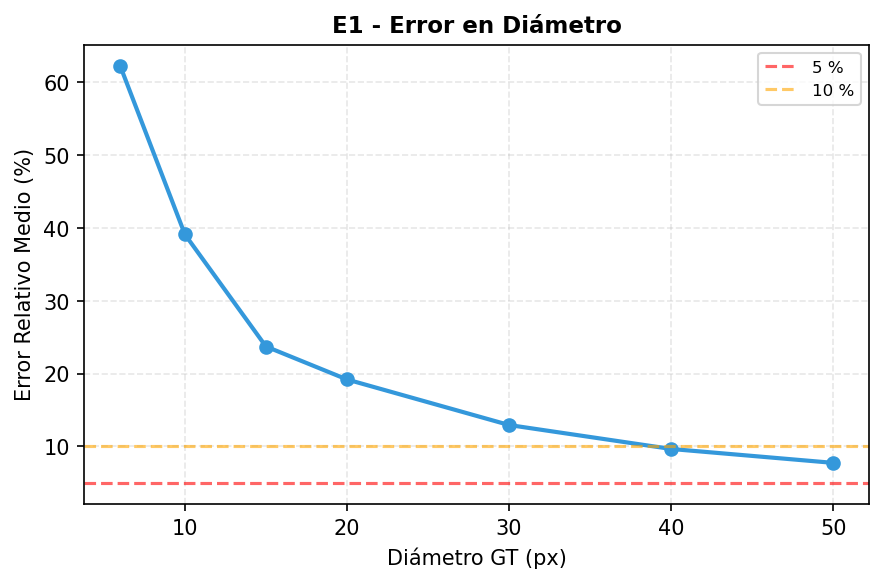
\includegraphics[width=\textwidth]{figures/tests/E1/E1_mre_diam.png}
    \end{subfigure}
    \begin{subfigure}[b]{0.7\textwidth}
        \centering
        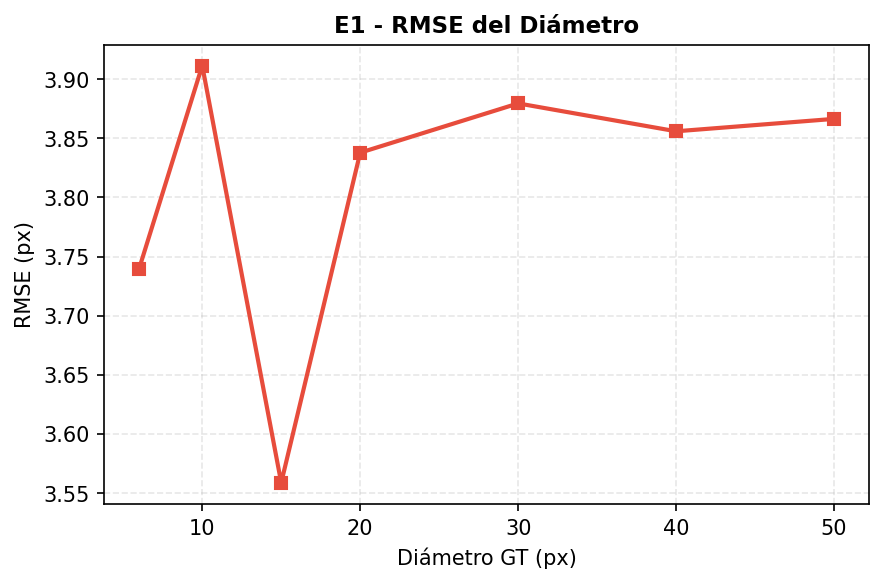
\includegraphics[width=\textwidth]{figures/tests/E1/E1_rmse_diam.png}
    \end{subfigure}
    \begin{subfigure}[b]{0.7\textwidth} 
        \centering
        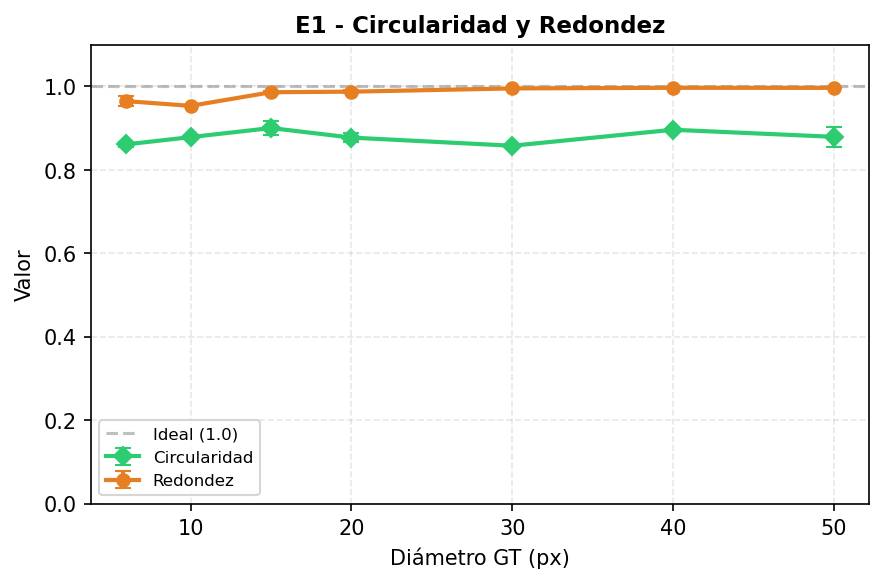
\includegraphics[width=\textwidth]{figures/tests/E1/E1_shape_metrics.png}
    \end{subfigure}
    
    \caption{Métricas de error de diámetro y forma para el experimento E1.}
    \label{fig:E1_metrics}
\end{figure}

\subsection{E2 - Precisión en la estimación de velocidad}
 
\textbf{Configuración:} Se generaron 5 vídeos de 60 frames con una única gota de 20~px de diámetro moviéndose a velocidad constante y conocida, cubriendo movimientos horizontal, vertical y diagonal en ambos sentidos, con magnitudes entre 2 y $\sqrt{4^2+2^2} \approx 4.5$~px/frame. La velocidad real de los experimentos de nebulización es del orden de miles de µm/ms, lo que a la escala del vídeo y con la tasa de adquisición usada equivale a pocos píxeles por frame; este rango es, por tanto, representativo.

\begin{table}[H]
\centering
\small
\caption{Resultados del experimento E2 (precisión de la estimación de velocidad y tracking). La velocidad se expresa en píxeles por frame (px/f).}
\begin{tabular}{ccccccc}
\hline
\textbf{($v_x, v_y$)} & \textbf{Velocidad GT} & \textbf{Velocidad Det.} & \textbf{MRE\textsubscript{vel} (\%)} & \textbf{RMSE\textsubscript{vel}} & \textbf{F1 Track} & \textbf{Frag.} \\
\hline
(2.0, 0.0)  & 2.000 px/f & 2.001 $\pm$ 0.018 px/f & 0.44 & 0.0090 px/f & 1.0 & 0.0 \\
(5.0, 0.0)  & 5.000 px/f & 5.001 $\pm$ 0.015 px/f & 0.12 & 0.0029 px/f & 1.0 & 0.0 \\
(0.0, 3.0)  & 3.000 px/f & 3.001 $\pm$ 0.014 px/f & 0.19 & 0.0045 px/f & 1.0 & 0.0 \\
(3.0, 3.0)  & 4.243 px/f & 4.244 $\pm$ 0.038 px/f & 0.45 & 0.0088 px/f & 1.0 & 0.0 \\
(-4.0, 2.0) & 4.472 px/f & 4.472 $\pm$ 0.013 px/f & 0.17 & 0.0029 px/f & 1.0 & 0.0 \\
\hline
\end{tabular}
\label{tab:e2_resultados}
\end{table}
 

\begin{figure}[htbp]
    \centering
        
    \begin{subfigure}[b]{0.85\textwidth}
        \centering
        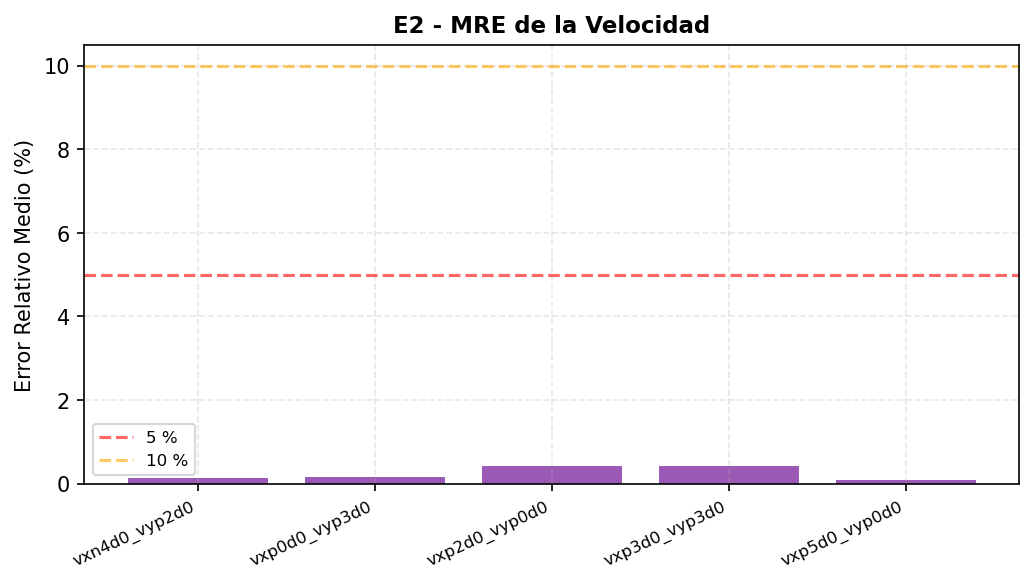
\includegraphics[width=\textwidth]{figures/tests/E2/E2_mre_vel.png}
    \end{subfigure}
    \begin{subfigure}[b]{0.85\textwidth}
        \centering
        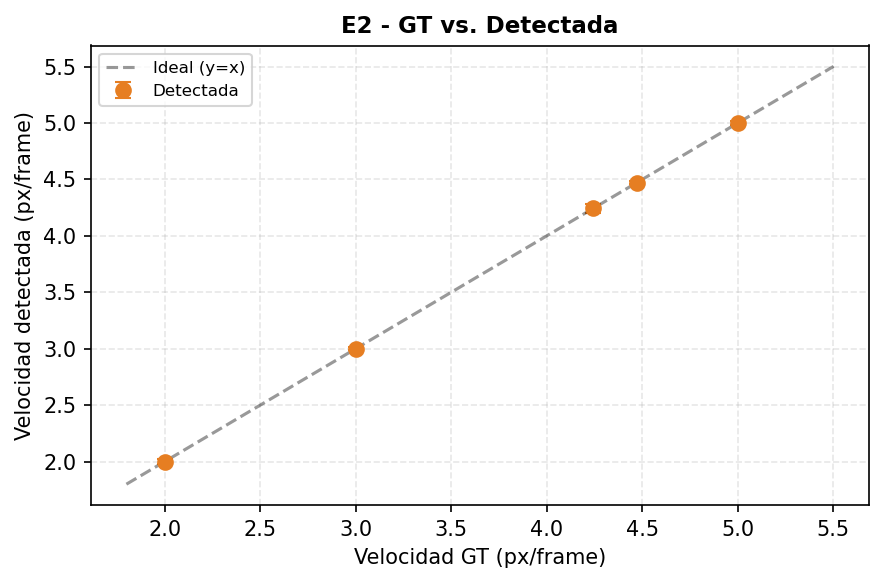
\includegraphics[width=\textwidth]{figures/tests/E2/E2_gt_vs_det.png}
    \end{subfigure}

    \caption{Métricas de error de velocidad para el experimento E2.}
    \label{fig:E2_metrics}
\end{figure}

En los datos mostrados en la tabla \ref{tab:e2_resultados} y en la figura \ref{fig:E2_metrics}, se aprecia que el analizador detecta la trayectoria completa y sin fragmentación (F1 de tracking de 1.0 y tasa de fragmentación de 0.0) en todos los casos. Por otro lado, el error relativo medio en la velocidad estimada es inferior al 0.5\% en todos los casos. Todo esto demuestra el excelente desempeño del analizador bajo condiciones sin ruido y con gota de tamaño moderado.


\subsection{E3 - Robustez al ruido}
 
\textbf{Configuración:} Se usó una única gota estática de 20~px de diámetro, evaluada bajo dos tipos de degradación de forma independiente: (a) ruido gaussiano aditivo con $\sigma \in \{0, 5, 10, 20, 35, 50\}$ y (b) ruido de tipo sal y pimienta con fracción de píxeles afectados $\in \{0\%, 2\%, 5\%, 10\%\}$. Este experimento permite caracterizar la sensibilidad del pipeline de preprocesamiento y segmentación ante condiciones de imagen degradada, habituales en los vídeos de alta velocidad donde la limitación de luz provoca un mayor nivel de ruido electrónico en el sensor.

\begin{figure}[H]
    \centering
    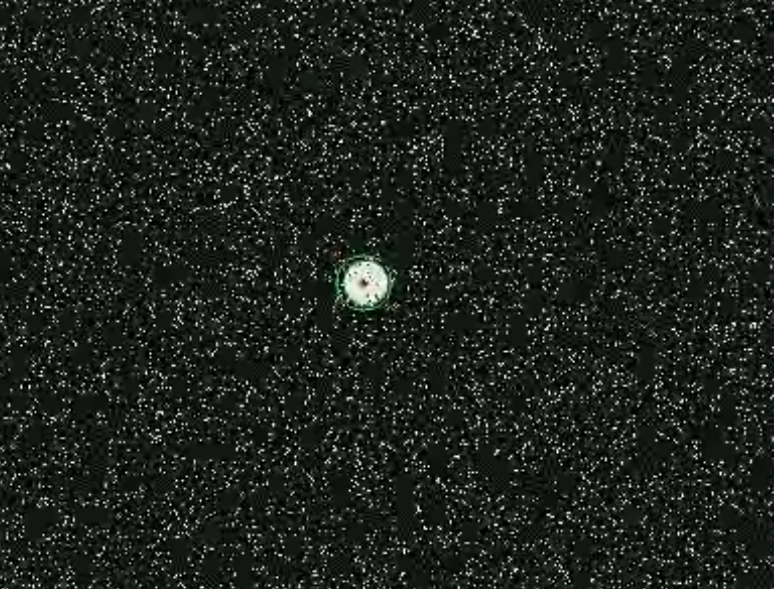
\includegraphics[width=0.4\textwidth]{figures/E3.png}
    \caption{Ejemplo de degradación por sal y pimienta al 10\%}
\end{figure}

\begin{table}[H]
\centering
\small
\caption{Resultados del experimento E3 (robustez al ruido gaussiano y sal y pimienta en gotas de 20 px).}
\begin{tabular}{lrccccc}
\hline
\textbf{Tipo de Ruido} & \textbf{Nivel} & \textbf{Recall} & \textbf{F1} & \textbf{MRE\textsubscript{diam} (\%)} & \textbf{RMSE\textsubscript{diam} (px)} & \textbf{Circ. media} \\
\hline
\multicolumn{7}{c}{\textit{Ruido Gaussiano ($\sigma$)}} \\
\hline
Gaussiano & 0  & 1.00 & 1.00 & 43.06 & 8.61 & 0.9291 \\
Gaussiano & 5  & 1.00 & 1.00 & 43.25 & 8.65 & 0.8766 \\
Gaussiano & 10 & 1.00 & 1.00 & 44.54 & 8.91 & 0.8284 \\
Gaussiano & 20 & 1.00 & 1.00 & 45.79 & 9.16 & 0.7900 \\
Gaussiano & 35 & 1.00 & 1.00 & 46.14 & 9.23 & 0.6930 \\
Gaussiano & 50 & 0.98 & 0.99 & 45.85 & 9.17 & 0.5526 \\
\hline
\multicolumn{7}{c}{\textit{Ruido Sal y Pimienta}} \\
\hline
Sal y Pimienta & 0\%  & 1.00 & 1.00 & 43.06 & 8.61 & 0.9291 \\
Sal y Pimienta & 2\%  & 1.00 & 1.00 & 43.50 & 8.70 & 0.8545 \\
Sal y Pimienta & 5\%  & 1.00 & 1.00 & 44.55 & 8.91 & 0.7652 \\
Sal y Pimienta & 10\% & 0.95 & 0.97 & 44.34 & 8.87 & 0.6100 \\
\hline
\end{tabular}
\label{tab:e3_resultados}
\end{table}

Como compromiso de diseño, se ha priorizado la detección y localización de las gotas por encima de la precisión de su diámetro. Esta severa reducción de ruido distorsiona y erosiona los contornos originales, provocando una pérdida de píxeles que infla el error absoluto del diámetro medido (RMSE\textsubscript{diam} $\approx$ 8.6 - 9.2 px) y deteriora de forma progresiva la métrica de circularidad debido a la irregularidad de los bordes resultantes. Sin embargo, esta estrategia asegura el éxito del tracking: la métrica F1 se mantiene excepcionalmente robusta y muy por encima del 90\% (superando el 97\% incluso en los escenarios críticos de $\sigma=50$ y $10\%$ de píxeles corruptos). Cabe destacar que se podría haber optado por una configuración de filtrado menos conservadora para mantener un diámetro más preciso; no obstante, dicha alternativa habría implicado perder la pista de numerosas gotas enmascaradas por el ruido (falsos negativos), hundiendo la tasa de recuperación (Recall) y comprometiendo el análisis de trayectorias.

\begin{figure}[H]
    \centering
        
    \begin{subfigure}[b]{0.7\textwidth}
        \centering
        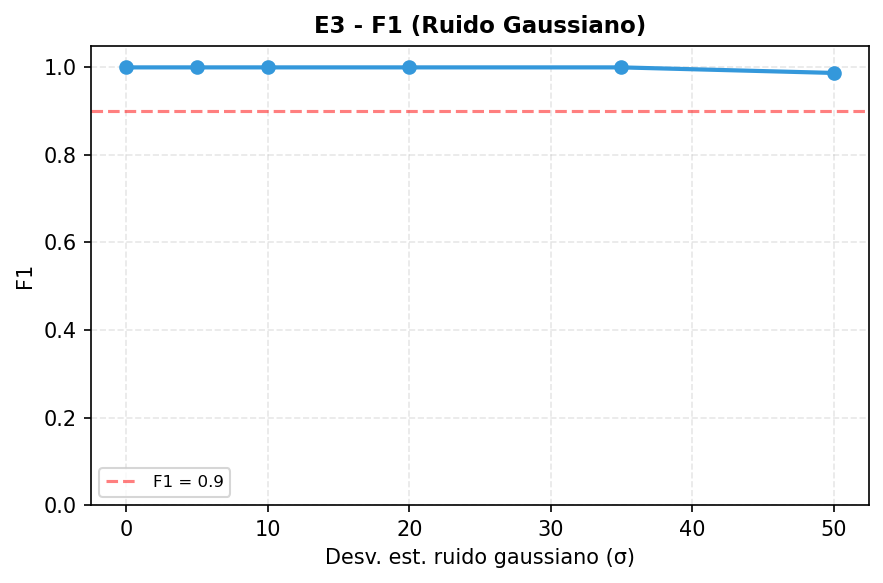
\includegraphics[width=\textwidth]{figures/tests/E3/E3_gauss_f1.png}
    \end{subfigure}
    \begin{subfigure}[b]{0.7\textwidth}
        \centering
        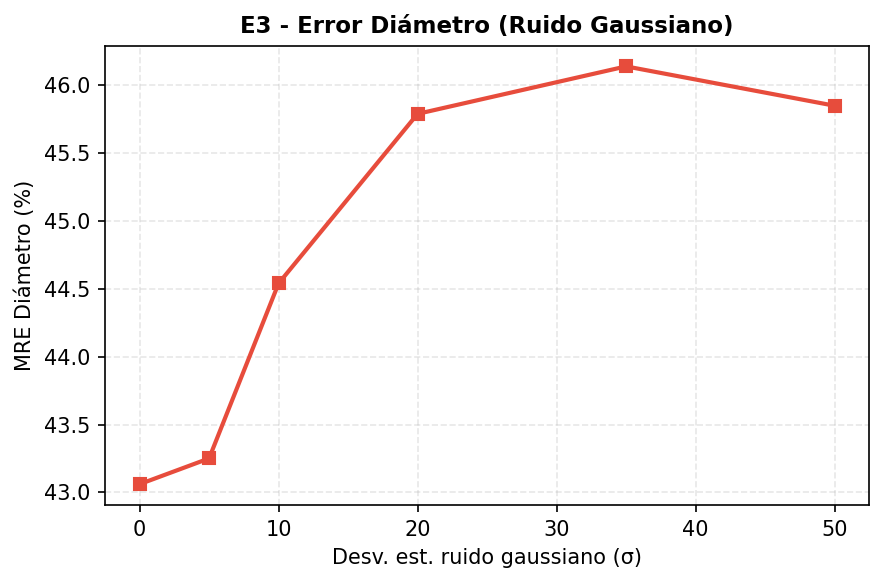
\includegraphics[width=\textwidth]{figures/tests/E3/E3_gauss_mre.png}
    \end{subfigure}

    \caption{Métricas de robustez al ruido gaussiano para el experimento E3.}
    \label{fig:E3_metrics_gauss}
\end{figure}

\begin{figure}[H]
    \centering
        
    \begin{subfigure}[b]{0.7\textwidth}
        \centering
        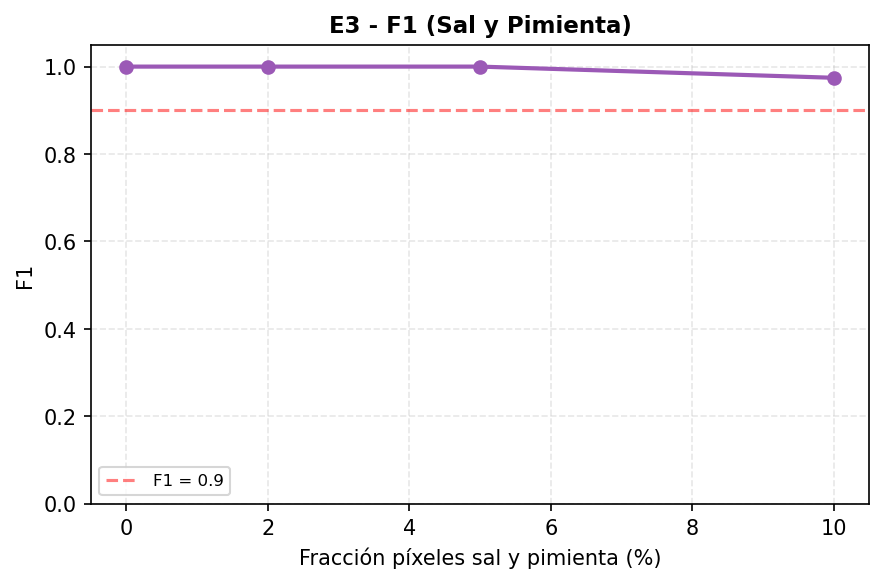
\includegraphics[width=\textwidth]{figures/tests/E3/E3_sp_f1.png}
    \end{subfigure}
    \begin{subfigure}[b]{0.7\textwidth}
        \centering
        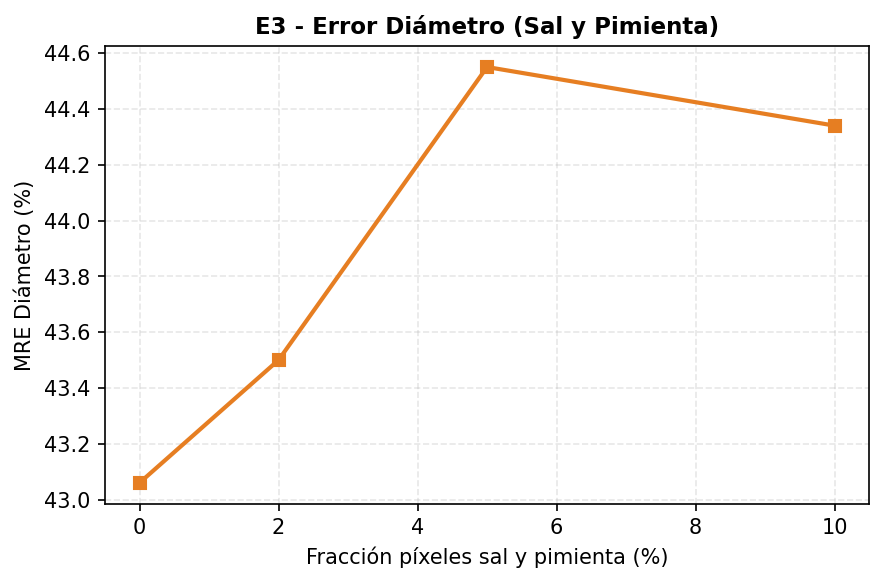
\includegraphics[width=\textwidth]{figures/tests/E3/E3_sp_mre.png}
    \end{subfigure}

    \caption{Métricas de robustez al ruido de tipo sal y pimienta para el experimento E3.}
    \label{fig:E3_metrics_sp}
\end{figure}

\subsection{E4 - Rango de tamaños detectables}
 
\textbf{Configuración:} Se generó un vídeo por cada diámetro del barrido $\{3, 4, 5, 6, 8, 10, 12, 15, 20, 25, 30, 40, 50, 60, 70, 80\}$~px, con una única gota centrada en el frame y ruido gaussiano de $\sigma = 8$ para simular condiciones realistas. Este experimento permite determinar el \textbf{límite inferior} de detección (diámetro mínimo fiable) y el \textbf{límite superior} (a partir del cual el área supera el umbral máximo configurado).

\begin{table}[H]
\centering
\small
\caption{Resultados del experimento E4 (Rango de tamaños detectables). Se omitió la columna Precision porque mantuvo un valor constante de 1.0 en todos los escenarios.}
\begin{tabular}{cccccc}
\hline
\textbf{Diámetro GT (px)} & \textbf{Recall} & \textbf{F1} & \textbf{MRE\textsubscript{diam} (\%)} & \textbf{RMSE\textsubscript{diam} (px)} & \textbf{Circ. media} \\
\hline
3  & 0.80 & 0.89 & 178.95 & 5.38 & 0.7134 \\
4  & 0.93 & 0.97 & 135.23 & 5.42 & 0.7291 \\
5  & 0.97 & 0.98 & 107.95 & 5.40 & 0.6876 \\
6  & 0.97 & 0.98 & 91.45  & 5.49 & 0.6943 \\
8  & 0.97 & 0.98 & 68.41  & 5.48 & 0.6870 \\
10 & 0.90 & 0.95 & 54.46  & 5.45 & 0.6736 \\
12 & 0.97 & 0.98 & 45.01  & 5.40 & 0.7042 \\
15 & 0.97 & 0.98 & 36.69  & 5.51 & 0.6830 \\
20 & 1.00 & 1.00 & 27.83  & 5.57 & 0.7238 \\
25 & 1.00 & 1.00 & 22.21  & 5.55 & 0.7360 \\
30 & 1.00 & 1.00 & 18.55  & 5.57 & 0.7847 \\
40 & 1.00 & 1.00 & 14.15  & 5.66 & 0.7949 \\
50 & 1.00 & 1.00 & 11.22  & 5.61 & 0.8282 \\
60 & 1.00 & 1.00 & 9.24   & 5.55 & 0.8356 \\
70 & 1.00 & 1.00 & 7.84   & 5.49 & 0.8389 \\
80 & 1.00 & 1.00 & 6.99   & 5.60 & 0.8376 \\
\hline
\end{tabular}
\label{tab:e4_resultados}
\end{table}

El sistema demuestra una excelente capacidad de localización incluso en el límite inferior. La métrica Recall supera el umbral de viabilidad (0.80) desde las gotas más diminutas de 3 px, y alcanza una recuperación perfecta (Recall = 1.0 y F1 = 1.0) de forma sostenida a partir de los 20 px. Al igual que en los experimentos anteriores, la precisión de la detección de presencia de gotas se desvincula de la fidelidad geométrica: el algoritmo presenta un ensanchamiento perimetral constante evidenciado por un error absoluto altamente estable (RMSE\textsubscript{diam} $\approx$ 5.5 px). Como se aprecia claramente en el gráfico del error de medición \ref{fig:E4_metrics}, este sesgo sistemático provoca una degradación del MRE\textsubscript{diam}, limitando la precisión para las gotas inferiores a 20 px. No obstante, para gotas medianas y grandes, el error relativo cae rápidamente por debajo de la cota del 10\%, validando el método para conteo en todo el espectro de tamaños y ofreciendo mediciones geométricas fiables para las gotas de un tamaño medio.

\begin{figure}[H]
    \centering
        
    \begin{subfigure}[b]{0.85\textwidth}
        \centering
        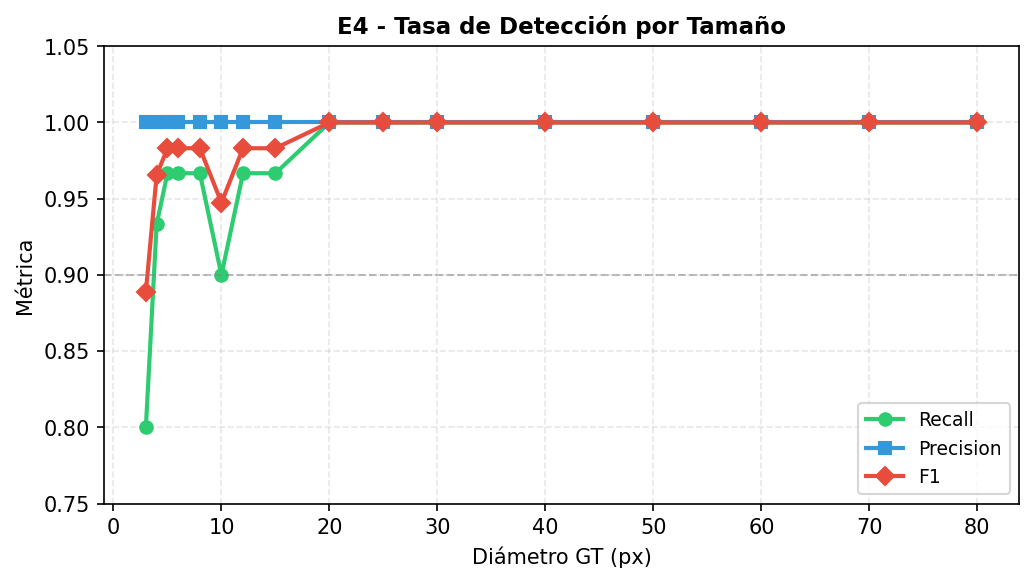
\includegraphics[width=\textwidth]{figures/tests/E4/E4_detection_rates.png}
    \end{subfigure}
    \begin{subfigure}[b]{0.85\textwidth}
        \centering
        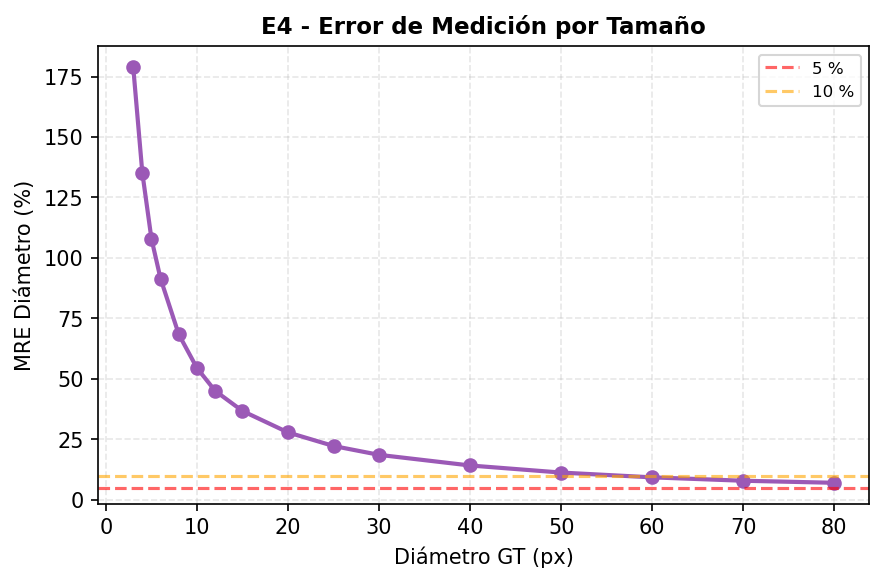
\includegraphics[width=\textwidth]{figures/tests/E4/E4_mre_diam.png}
    \end{subfigure}

    \caption{Métricas del experimento E4 (Rango de tamaños detectables).}
    \label{fig:E4_metrics}
\end{figure}

\subsection{E5 - Impacto de la densidad de gotas en el tracking}
 
\textbf{Configuración:} Se generaron vídeos de 60 frames con $N \in \{5, 10, 20, 35, 50\}$ gotas de 18~px de diámetro moviéndose simultáneamente a 3~px/frame en direcciones aleatorias (semilla fija para reproducibilidad), con ruido gaussiano de $\sigma = 8$. A mayor densidad, aumenta la probabilidad de oclusiones y de que el tracker asigne erróneamente la identidad de una gota a otra.

\begin{table}[H]
\centering
\small
\caption{Resultados del experimento E5 (impacto de la densidad de gotas en el tracking y la estimación cinemática). La Precision se omite por mantenerse constante en 1.0.}
\begin{tabular}{cccccc}
\hline
\textbf{Densidad ($N$)} & \textbf{Recall} & \textbf{F1} & \textbf{Fragmentación} & \textbf{MRE\textsubscript{vel} (\%)} & \textbf{RMSE\textsubscript{vel} (px/f)} \\
\hline
5  & 0.95 & 0.97 & 0.00 & 5.34  & 0.07 \\
10 & 0.91 & 0.95 & 0.10 & 5.47  & 0.09 \\
20 & 0.87 & 0.93 & 0.35 & 9.47  & 0.71 \\
35 & 0.81 & 0.89 & 0.31 & 16.90 & 1.12 \\
50 & 0.74 & 0.85 & 0.28 & 45.48 & 2.28 \\
\hline
\end{tabular}
\label{tab:e5_resultados}
\end{table}

En la Tabla \ref{tab:e5_resultados} y las figuras \ref{fig:E5_metrics} se cuantifica el deterioro del rendimiento del algoritmo a medida que aumenta la densidad de partículas. Como era previsible, el incremento en la concentración induce un mayor número de oclusiones espaciales, provocando una caída monótona en la tasa de recuperación (Recall), que desciende desde un excelente 0.95 con 5 gotas hasta un 0.74 en el escenario de máxima congestión (50 gotas). El efecto más perjudicial recae sobre el módulo de tracking y la estimación cinemática: a partir de las 20 gotas simultáneas, la tasa de fragmentación de trayectorias sufre un incremento abrupto (0.35). Esto indica que el algoritmo pierde la pista de las partículas durante los cruces y corrompe el cálculo temporal del desplazamiento, disparando el error relativo de la velocidad (MRE\textsubscript{vel}) por encima del $45\%$ en densidades extremas. No obstante, es crucial contextualizar estos resultados: en esta simulación sintética, las partículas se mueven en direcciones totalmente aleatorias, un diseño planteado ex profeso para someter al sistema a una prueba de estrés en el peor escenario posible. En un ensayo físico real de nebulización, el flujo posee una marcada direccionalidad, con la inmensa mayoría de las gotas viajando en el mismo sentido desde el inyector hacia el exterior. Esta coherencia vectorial reduce drásticamente la probabilidad geométrica de trayectorias cruzadas en comparación con el modelo sintético. Por tanto, aunque las estimaciones cinemáticas deben evaluarse con cautela en el núcleo más denso del aerosol, el rendimiento y la continuidad del tracker en condiciones reales de laboratorio serán previsiblemente superiores a los reportados en este límite teórico.

\begin{figure}[H]
    \centering
        
    \begin{subfigure}[b]{0.7\textwidth}
        \centering
        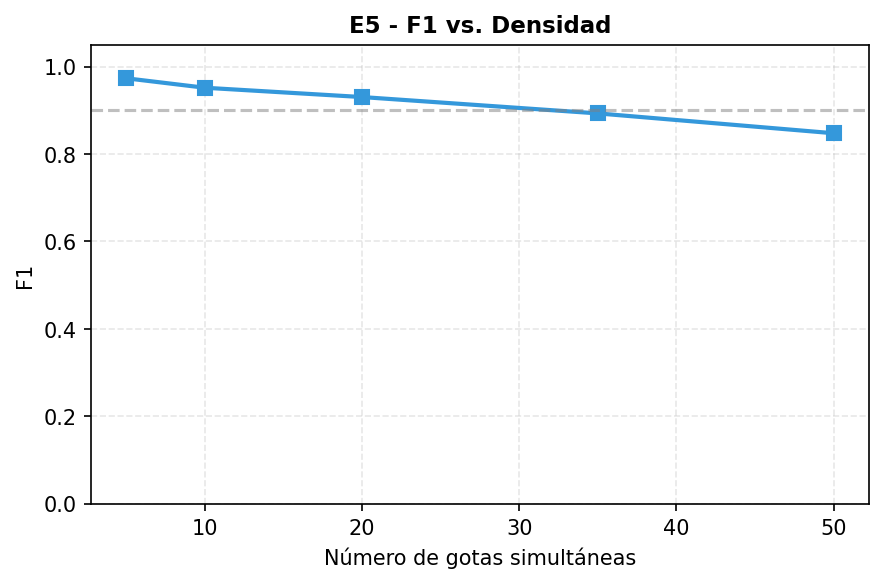
\includegraphics[width=\textwidth]{figures/tests/E5/E5_f1.png}
    \end{subfigure}
    \begin{subfigure}[b]{0.7\textwidth}
        \centering
        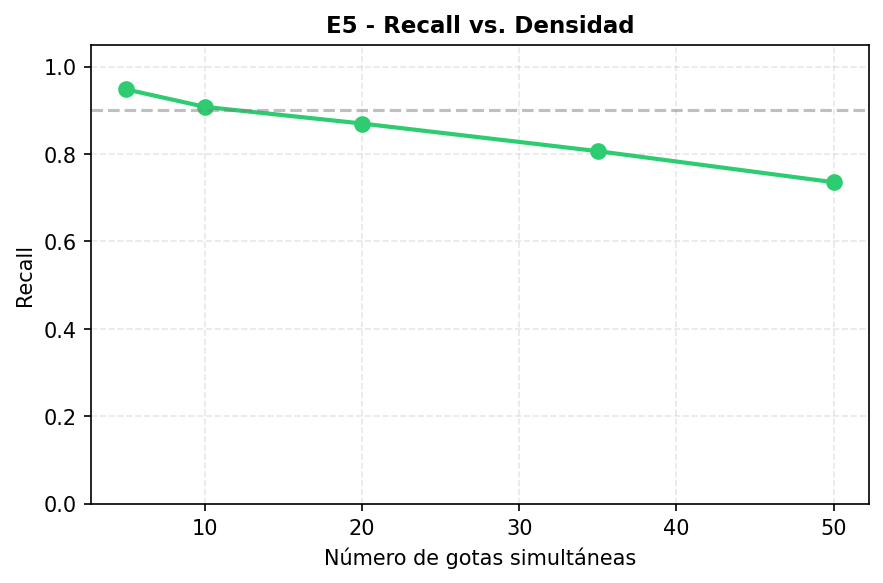
\includegraphics[width=\textwidth]{figures/tests/E5/E5_recall.png}
    \end{subfigure}
    \begin{subfigure}[b]{0.7\textwidth} 
        \centering
        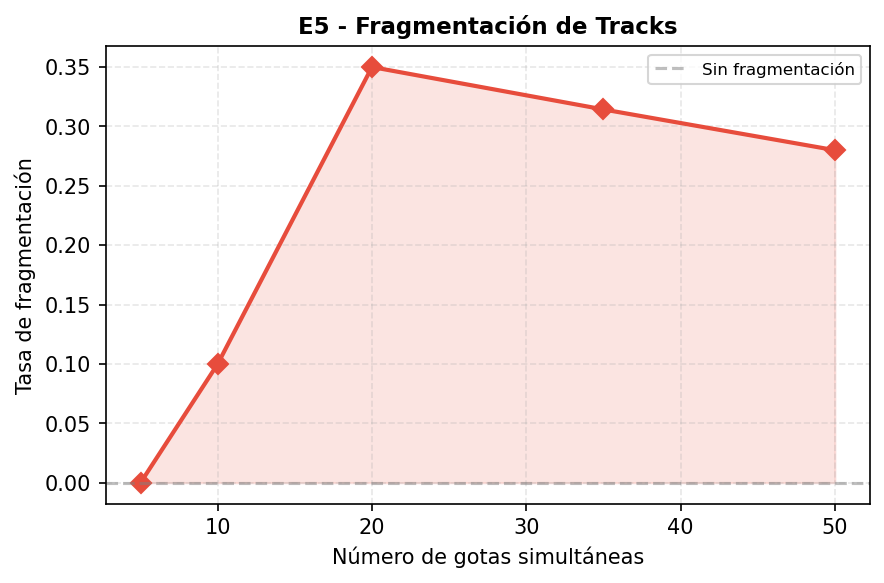
\includegraphics[width=\textwidth]{figures/tests/E5/E5_frag_rate.png}
    \end{subfigure}
    
    \caption{Métricas del experimento E5 (impacto de la densidad de gotas en el tracking y la estimación cinemática).}
    \label{fig:E5_metrics}
\end{figure}

\section{Evaluación cualitativa}

La evaluación cuantitativa sobre vídeos sintéticos valida la precisión del sistema bajo condiciones controladas, pero no garantiza su correcto funcionamiento con los vídeos reales de los experimentos de nebulización, que presentan características distintas: iluminación no uniforme, gotas desenfocadas en distintos planos, presencia del anillo circular del objetivo de la cámara y movimientos más complejos.

Para evaluar el desempeño del analizador en condiciones reales, se han procesado varios vídeos de experimentos de nebulización realizados en el laboratorio. En la figura \ref{fig:real_video} se muestra un frame de uno de estos vídeos, con las detecciones y tracks superpuestos.

\begin{figure}[H]
    \centering
    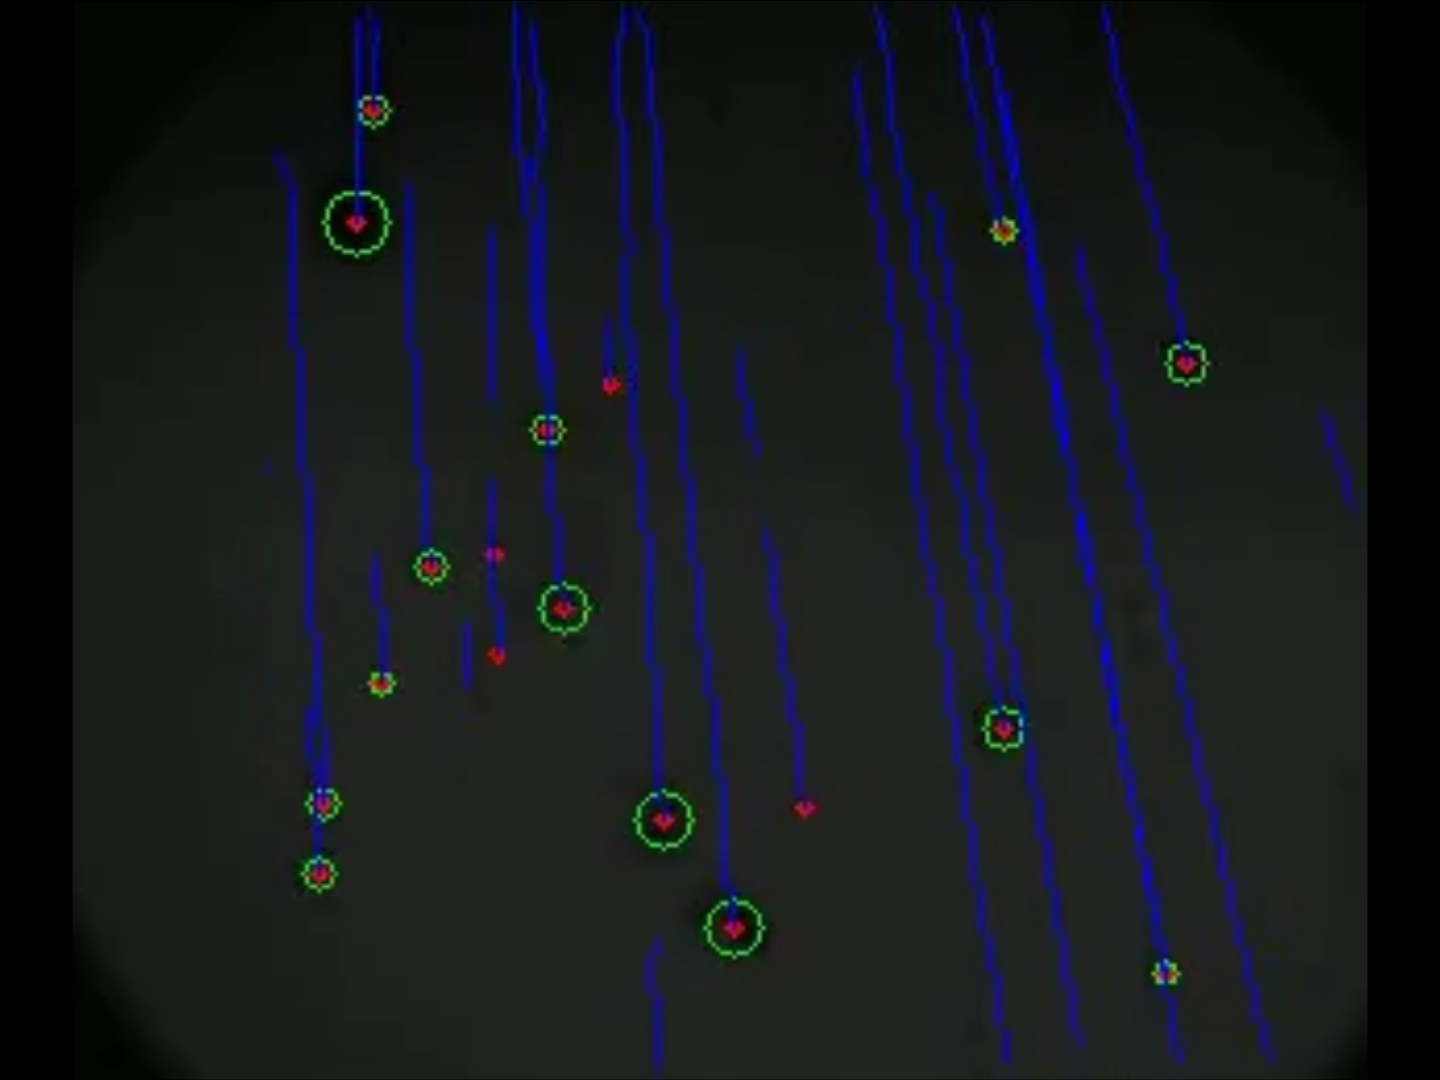
\includegraphics[width=0.8\textwidth]{figures/cuali.png}
    \caption{Frame de un vídeo real procesado por el analizador. Las detecciones se muestran como círculos verdes y los tracks como líneas de colores.}
    \label{fig:real_video}
\end{figure}

En el frame anterior se puede apreciar que pese a la baja calidad del vídeo se consiguen extraer la mayoría de las gotas junto con sus trayectorias. Además, las trayectorias marcadas, no poseen apenas discontinuidades, lo que indica que el analizador ha sido capaz de seguir el rastro de las gotas. Hay que decir, que hay gotas que no se detectan debido a la mala iluminación, el desenfoque y la oclusión, pero el sistema nos da una aproximación general de la dinámica del spray.